\documentclass[border=4pt]{standalone}
\usepackage[T1]{fontenc}
\usepackage{helvet}
\renewcommand{\familydefault}{\sfdefault}
\usepackage{graphicx}
\usepackage{caption}
\usepackage{amsmath}
\captionsetup{font={sf,footnotesize},labelfont={sf,bf,footnotesize},justification=justified,singlelinecheck=false}
\begin{document}
\setcounter{figure}{8}
\begin{minipage}{7.20in}
\centering
\begin{figure}[htbp]
    \centering
    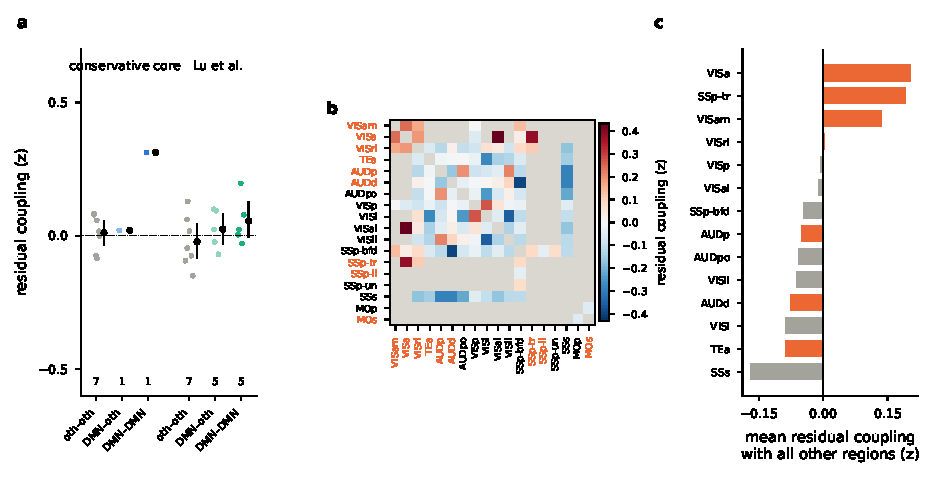
\includegraphics[width=\linewidth]{fig9_meso_panels.pdf}
    \caption{\textbf{a} Mesoscope, inter-trial rest (the grey screen images RSP in only 1--2 mice): still 1 s bins from 1 s after feedback to 0.2 s before the next stimulus, nuisance-regressed; RSP pairs from 14 sessions, 5 mice. The mesoscope images no frontal core region, so the core is RSPagl and RSPd. Residual coupling (distance-matched) per pair class, averaged per mouse (dots; number of mice at the bottom); black, mean and 95\% bootstrap CI where $\geq$3 mice. \textbf{b} Mean residual coupling of RSP with each imaged region (pairs in $\geq$2 mice; numbers above bars: mice), coloured as in Fig. 4.}
    \label{fig:grey_meso}
\end{figure}
\end{minipage}
\end{document}
